\documentclass[a4paper, 12 pt]{article}
\usepackage[left=2cm, right=2cm, top=2cm]{geometry}
\usepackage{array}
\usepackage{color}
\usepackage{graphicx}
\usepackage{float}
\begin{document}
\centering
{\Huge\textcolor{blue}{\bf Raj Kumar Bhagat}}\\
\rule{18cm}{0.1pt}
\begin{table}[h]
\begin{tabular}{p{11 cm}p{6cm}}
Room Number 56,& contact : 9973048519\\
Amber-A Hostel,& emailid : rajk55460@gmail.com\\
NIT Tiruchirappalli Campus,\\
Tamil Nadu - 620015
\end{tabular}
\end{table}
% inserting images
\begin{figure}[H]
\raggedleft
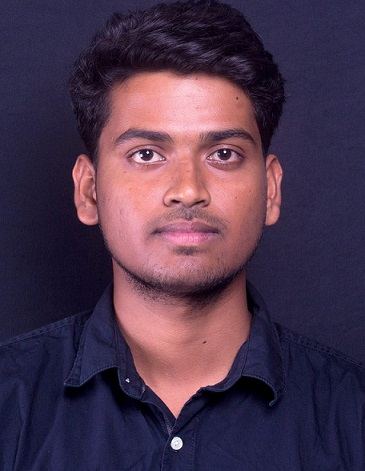
\includegraphics[scale=0.3]{Rajk0520.jpg}
\end{figure}
\raggedright
% inserting odjective
\section*{Objective :}
Currently a second year undergrad at NIT Trichy, I aspire to be a successful Research and Development Engineer with sufficient technical and social skills to contribute in the development of our nation.
% inserting education
\section*{Education :}
\begin{table}[h]
\begin{tabular}{|p{3.5 cm}|p{5.5cm}|p{3 cm}|p{4cm}|}
\hline
\bf Degree& \bf School/University& \bf Passing Year& \bf Percentage/CGPA\\
\hline
B.Tech&NIT Tiruchirappalli, Tamil Nadu&2021&CGPA : 8.41(till now) \\
\hline
Higher Secondary Education (CBSE)&JVM Shyamali, Ranchi, Jharkhand&2017&91\% \\
\hline
Secondary Education (CBSE)&DAV Public School, Gumla, Jharkhand &2015&CGPA : 10\\
\hline
\end{tabular}
\end{table}
% inserting projects
\section*{Projects :}
\begin{itemize}
\item {\Large \textbf{Mocking Bot}}{ \hfill {\bf eYRC-2018, IIT Bombay}}\\
{\bf Audio Processing, Embedded System, Sensor Interfacing.} \hfill{\bf Nov 2018-Mar} \\ \hfill {\bf 2019}\\
To a given audio file apply audio processing. Extract the notes, onset, instrument from the audio. Communicate the information to the bot which will imitate the same music on piano and trumpet made for the same.
\item {\Large \textbf{Portable Braille}}{ \hfill {\bf Sangam'18, Pragyan, NIT Trichy}}\\
{\bf Embedded Systems, Image Processing, Circuit Design.}\hfill{\bf Dec 2018 - Mar} \\ \hfill {\bf 2019}\\
This project is an approach to solve the problem of unavailability of many of the books and texts in Braille scripts. In short, it is an assistive reading technology: Portable Braille, a system which is able to translate the captured image of a printed material into Braille code and reproduce them in the braille terminal.\\
\item {\Large \textbf{Wireless Gesture Controlled Game Controller }}\\
{\bf Embedded Systems, IR Communication, Sensor Interfacing.} \hfill {\bf Aug 2018-Sept}\\ \hfill {\bf 2018}\\
A wireless gesture recognition setup which is used in place of keyboard to play various games. This setup includes IR Communication (NEC Protocol), microcontroller etc.
\end{itemize}
% inserting projects
\section*{Technical Skills :}
\begin{itemize}
\item {\large {\bf Programming Language :}} C, Embedded C, C++, Python, Arduino, LaTex.
\item {\large {\bf Hardware :}} AtMega Series (AVR Microcontrollers), Arduino, Raspberry pi.
\item {\large {\bf Software Skills :}} Sonic Visualizer, MATLAB.
\end{itemize}
% inserting soft skills
\section*{Soft Skills :}
\begin{itemize}
\item Dedicated
\item Collaborative
\item Organization
\end{itemize}
% inserting soft skills
\section*{Extra-Curricular Activities :}
\begin{itemize}
\item Member (Embedded), at {\bf SPIDER, R\&D Club of NIT Trichy}.
\item Organizer at {\bf AAVEG’18}, first year inter-hostel fest of {\bf NIT Trichy}.
\item Workshop Coordinator at CURRENTS’19, {\bf EEE Department Symposium, NIT Trichy}.
\end{itemize}
\end{document}